\documentclass{beamer}
\usepackage[english, russian]{babel}
\usepackage[T2A]{fontenc}
\usepackage[utf8]{inputenc}
\usepackage{indentfirst}
\usepackage{amsmath, amsfonts, amssymb, amsthm, mathtools}
\usepackage[export]{adjustbox}
\usepackage{graphicx} 
\graphicspath{ {./images/} }

\usepackage{subcaption}
\usepackage{verbatim}

\usepackage{minted}{\setlength{\parskip}{0pt}}

\usepackage{hyperref}

\hypersetup{
    colorlinks=true,
    linkcolor=blue,
    filecolor=magenta,      
    urlcolor=black,
    pdftitle={Overleaf Example},
    pdfpagemode=FullScreen,
    }


\title{Отчет по лабораторной работе № 13. \\ Настройка NFS}
\author{Данила Стариков \\ НПИбд-02-22}
\date{2024}

\begin{document}

\maketitle
\newpage

\tableofcontents

\newpage
\section{Цель работы}
Приобретение навыков настройки сервера NFS для удалённого доступа к ресурсам.
\newpage

\section{Выполнение работы}
\subsection{Настройки сервера NFSv4}
\begin{enumerate}
\item На сервере установили необходимое программное обеспечение:
    \begin{minted}{bash}
dnf -y install nfs-utils
    \end{minted}
\item На сервере создали каталог, который предполагается сделать доступным всем
пользователям сети (корень дерева NFS):
    \begin{minted}{bash}
mkdir -p /srv/nfs
    \end{minted}
\item В файле /etc/exports прописали подключаемый через NFS общий каталог с доступом только на чтение:
    \begin{minted}{bash}
/srv/nfs *(ro)
    \end{minted}
\item Для общего каталога задали контекст безопасности NFS (Рис. \ref{img:01}):
    \begin{minted}{bash}
semanage fcontext -a -t nfs_t "/srv/nfs(/.*)?"
    \end{minted}
\item Применили изменённую настройку SELinux к файловой системе (Рис. \ref{img:01}):
    \begin{minted}{bash}
restorecon -vR /srv/nfs
    \end{minted}

\begin{center}
    \centering
    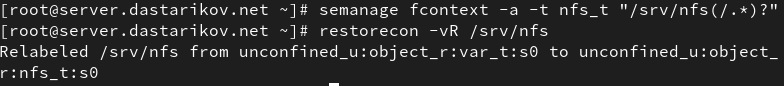
\includegraphics[width=\textwidth]{../images/image01.png}
    \captionof{figure}{Создание контекста безопасности для каталога /srv/nfs.}
    \label{img:01}
\end{center}

\item Запустили сервер NFS (Рис. \ref{img:02}):
    \begin{minted}{bash}
systemctl start nfs-server.service
systemctl enable nfs-server.service
    \end{minted}

\begin{center}
    \centering
    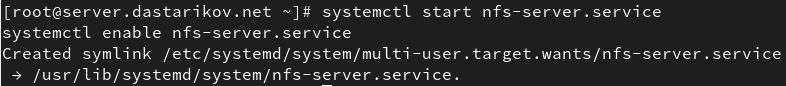
\includegraphics[width=\textwidth]{../images/image02.png}
    \captionof{figure}{Запуск сервера NFS.}
    \label{img:02}
\end{center}

\item Настроили межсетевой экран для работы сервера NFS (Рис. \ref{img:03}):
    \begin{minted}{bash}
firewall-cmd --add-service=nfs
firewall-cmd --add-service=nfs --permanent
firewall-cmd --reload
    \end{minted}

\begin{center}
    \centering
    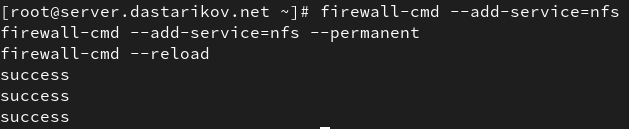
\includegraphics[width=\textwidth]{../images/image03.png}
    \captionof{figure}{Настройка межсетевого экрана.}
    \label{img:03}
\end{center}

\item На клиенте установили необходимое для работы NFS программное обеспечение:
    \begin{minted}{bash}
dnf -y install nfs-utils
    \end{minted}
\item На клиенте попробовали посмотреть имеющиеся подмонтированные удалённые
ресурсы (вместо dastarikov укажите свой логин) (Рис. \ref{img:04}):
    \begin{minted}{bash}
showmount -e server.dastarikov.net
    \end{minted}
В отчёте поясните, что при этом происходит.
\item Попробовали на сервере остановить сервис межсетевого экрана:
    \begin{minted}{bash}
systemctl stop firewalld.service
    \end{minted}
Затем на клиенте вновь попробовали подключиться к удалённо смонтированному ресурсу (Рис. \ref{img:04}):
    \begin{minted}{bash}
showmount -e server.dastarikov.net
    \end{minted}

\begin{center}
    \centering
    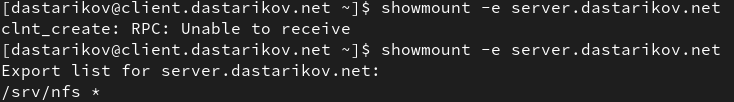
\includegraphics[width=\textwidth]{../images/image04.png}
    \captionof{figure}{Попытки подключения к удаленно смонтированному ресурсу.}
    \label{img:04}
\end{center}

% В отчёте поясните, что при этом происходит.
\item На сервере запустили сервис межсетевого экрана
    \begin{minted}{bash}
systemctl start firewalld
    \end{minted}
\item На сервере посмотрели, какие службы задействованы при удалённом монтировании (Рис. \ref{img:30} и \ref{img:31}):
    \begin{minted}{bash}
lsof | grep TCP
lsof | grep UDP
    \end{minted}

\begin{center}
    \centering
    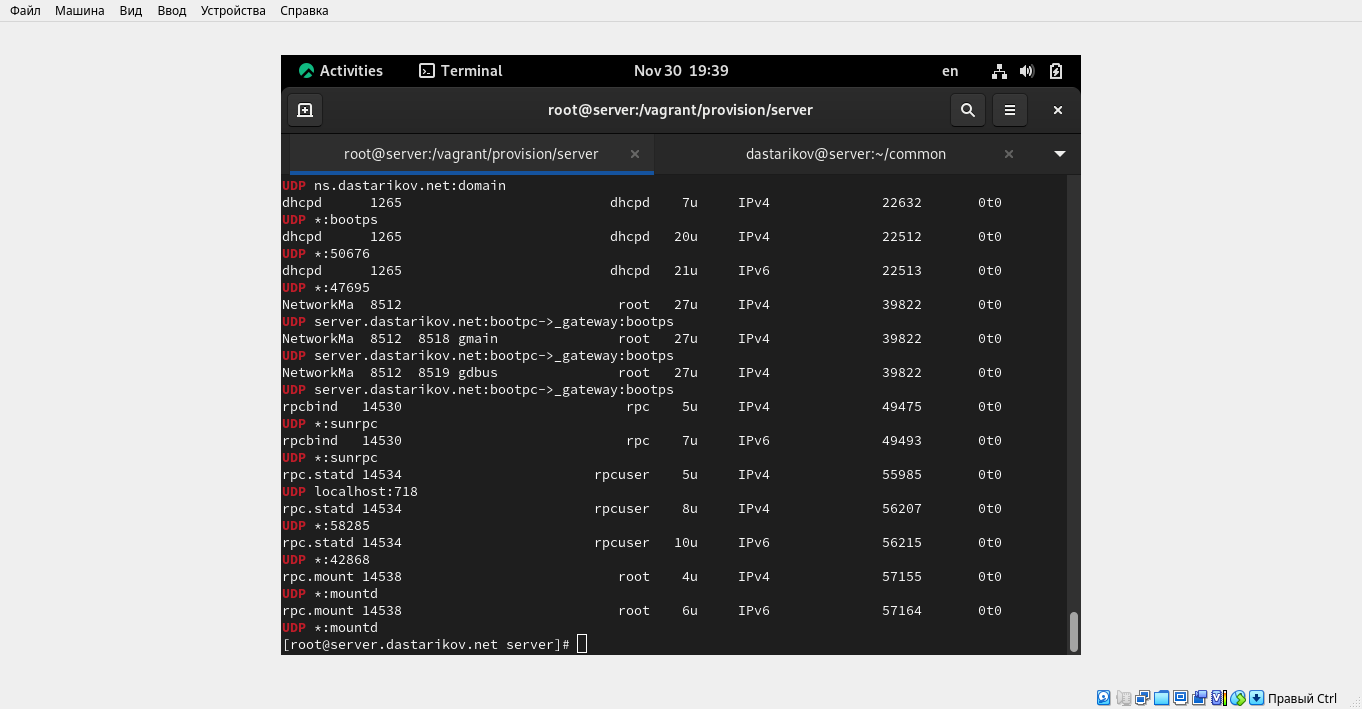
\includegraphics[width=\textwidth]{../images/image30.png}
    \captionof{figure}{Задействованные службы по протоколу UDP.}
    \label{img:30}
\end{center}
\begin{center}
    \centering
    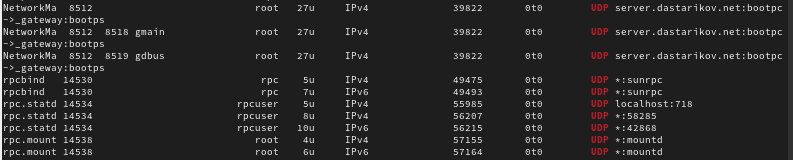
\includegraphics[width=\textwidth]{../images/image31.png}
    \captionof{figure}{Задействованные службы по протоколу TCP.}
    \label{img:31}
\end{center}
\item Добавили службы rpc-bind и mountd в настройки межсетевого экрана на сервере (Рис. \ref{img:05}):
    \begin{minted}{bash}
firewall-cmd --get-services
firewall-cmd --add-service=mountd --add-service=rpc-bind
firewall-cmd --add-service=mountd --add-service=rpc-bind --permanent
firewall-cmd --reload
    \end{minted}

\begin{center}
    \centering
    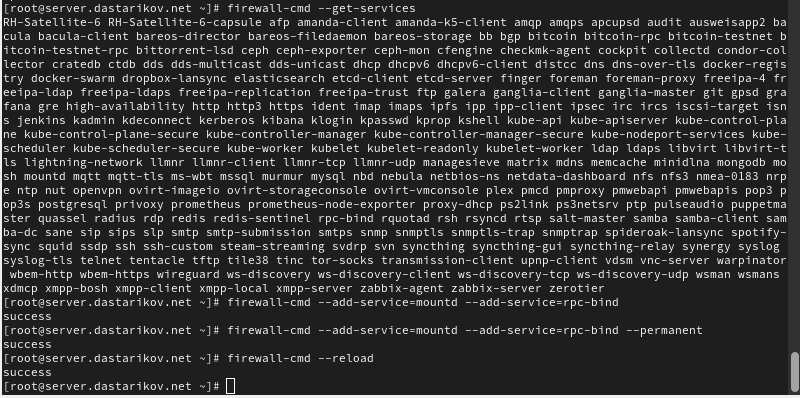
\includegraphics[width=\textwidth]{../images/image05.png}
    \captionof{figure}{Добавление служб rpc-bind и mountd в настройки межсетевого экрана.}
    \label{img:05}
\end{center}

\item На клиенте проверили подключение удалённого ресурса (Рис. \ref{img:06}):
    \begin{minted}{bash}
showmount -e server.dastarikov.net
    \end{minted}

\begin{center}
    \centering
    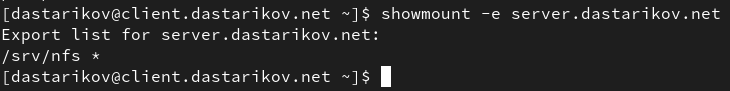
\includegraphics[width=\textwidth]{../images/image06.png}
    \captionof{figure}{Проверка подключения удаленного ресурса.}
    \label{img:06}
\end{center}

\end{enumerate}

\subsection{Монтирование NFS на клиенте}
\begin{enumerate}
\item На клиенте создали каталог, в который будет монтироваться удалённый ресурс, и подмонтировали дерево NFS (Рис. \ref{img:07}):
    \begin{minted}{bash}
mkdir -p /mnt/nfs
mount server.dastarikov.net:/srv/nfs /mnt/nfs
    \end{minted}

\begin{center}
    \centering
    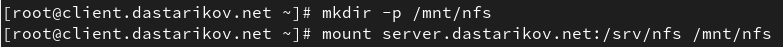
\includegraphics[width=\textwidth]{../images/image07.png}
    \captionof{figure}{Создание каталога на клиенте, в который будет монтироваться удаленный ресурс.}
    \label{img:07}
\end{center}

\item Проверили, что общий ресурс NFS подключён правильно (Рис. \ref{img:08}):
    \begin{minted}{bash}
mount
    \end{minted}

\begin{center}
    \centering
    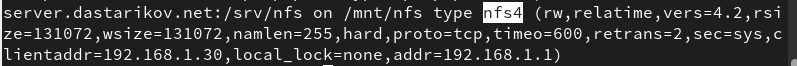
\includegraphics[width=\textwidth]{../images/image08.png}
    \captionof{figure}{Проверка правильности подключения ресурса NFS.}
    \label{img:08}
\end{center}

% В отчёте поясните выведенную информацию о монтировании удалённого ресурса.
\item На клиенте в конце файла /etc/fstab добавили следующую запись (Рис. \ref{img:09}):
    \begin{minted}{bash}
server.dastarikov.net:/srv/nfs /mnt/nfs nfs _netdev 0 0
    \end{minted}

\begin{center}
    \centering
    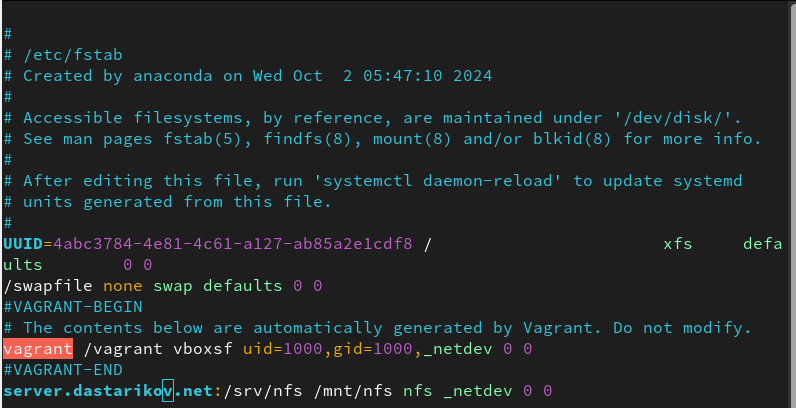
\includegraphics[width=\textwidth]{../images/image09.png}
    \captionof{figure}{Изменение файла /etc/fstab.}
    \label{img:09}
\end{center}

% В отчёте поясните синтаксис этой записи.
\item На клиенте проверили наличие автоматического монтирования удалённых ресурсов при запуске операционной системы (Рис. \ref{img:10}):
    \begin{minted}{bash}
systemctl status remote-fs.target
    \end{minted}

\begin{center}
    \centering
    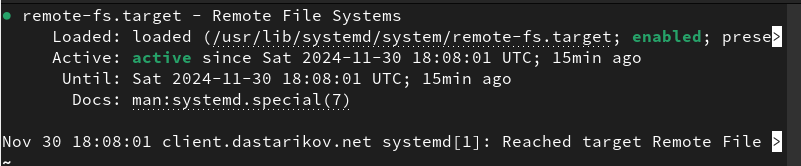
\includegraphics[width=\textwidth]{../images/image10.png}
    \captionof{figure}{Проверка автоматического монтирования удаленных ресурсов на клиенте.}
    \label{img:10}
\end{center}

\item Перезапустили клиента и убедились, что удалённый ресурс подключается автоматически (Рис. \ref{img:11}).

\begin{center}
    \centering
    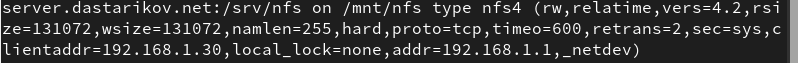
\includegraphics[width=\textwidth]{../images/image11.png}
    \captionof{figure}{Проверка автоматического монтирования после перезагрузки клиента.}
    \label{img:11}
\end{center}

\end{enumerate}

\subsection{Подключение каталогов к дереву NFS}
\begin{enumerate}
    \item На сервере создали общий каталог, в который затем будет подмонтирован каталог с контентом веб-сервера (Рис. \ref{img:15}):
    \begin{minted}{bash}
mkdir -p /srv/nfs/www
    \end{minted}
\item Подмонтировали каталог web-сервера:
    \begin{minted}{bash}
mount -o bind /var/www/ /srv/nfs/www/
    \end{minted}

\begin{center}
    \centering
    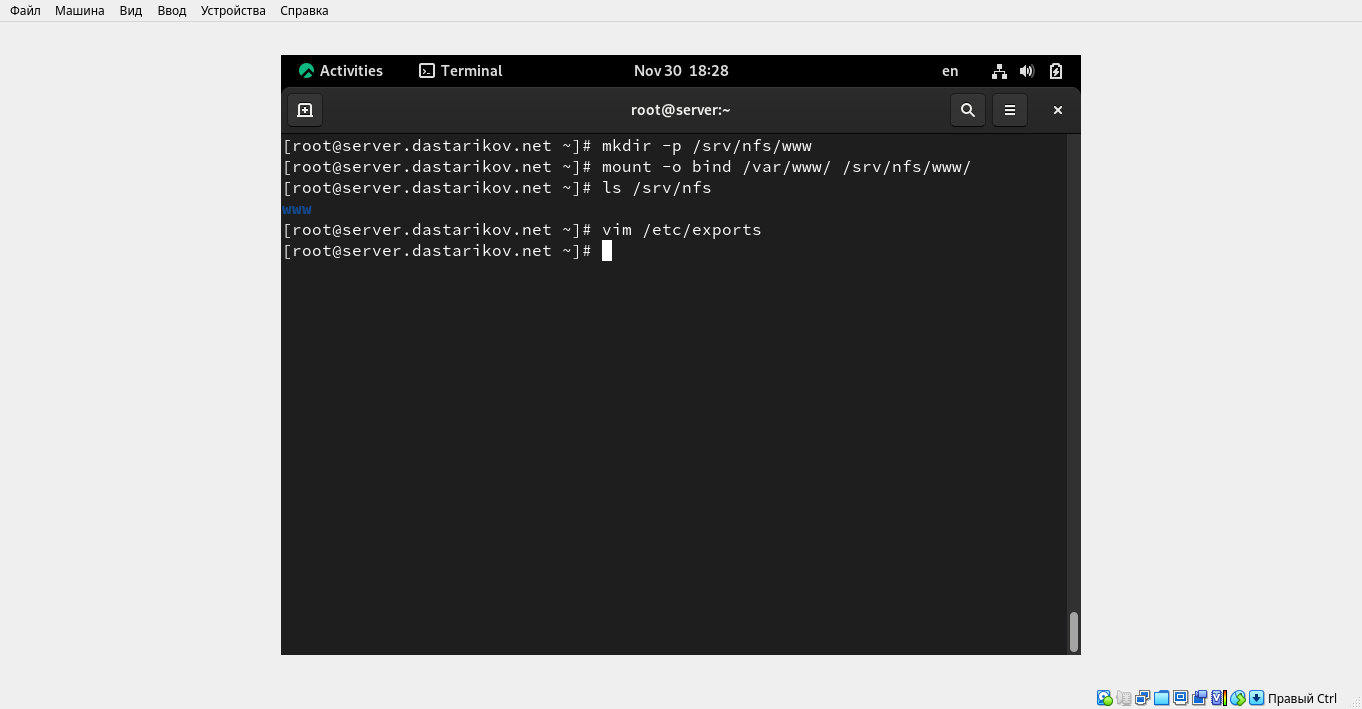
\includegraphics[width=\textwidth]{../images/image15.png}
    \captionof{figure}{Создание общего каталога с контентом веб-сервера.}
    \label{img:15}
\end{center}

\item На сервере проверили, что отображается в каталоге /srv/nfs (Рис. \ref{img:12}).

\begin{center}
    \centering
    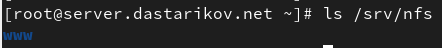
\includegraphics[width=\textwidth]{../images/image12.png}
    \captionof{figure}{Проверка содержимого /srv/nfs.}
    \label{img:12}
\end{center}

\item На клиенте посмотрели, что отображается в каталоге /mnt/nfs (Рис. \ref{img:13}).

\begin{center}
    \centering
    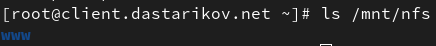
\includegraphics[width=\textwidth]{../images/image13.png}
    \captionof{figure}{Проверка содержимого /mnt/nfs.}
    \label{img:13}
\end{center}

\item На сервере в файле /etc/exports добавили экспорт каталога веб-сервера с удалённого ресурса (Рис. \ref{img:14}):
    \begin{minted}{bash}
/srv/nfs/www 192.168.0.0/16(rw)
    \end{minted}

\begin{center}
    \centering
    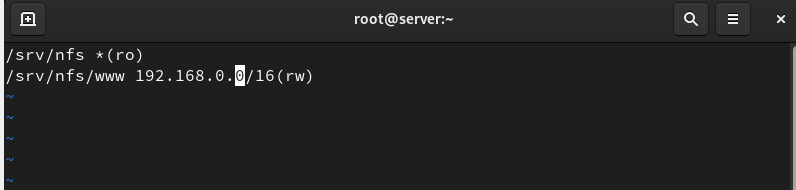
\includegraphics[width=\textwidth]{../images/image14.png}
    \captionof{figure}{Изменение файла /etc/exports.}
    \label{img:14}
\end{center}

\item Экспортировали все каталоги, упомянутые в файле /etc/exports:
    \begin{minted}{bash}
exportfs -r
    \end{minted}
\item Проверили на клиенте каталог /mnt/nfs.
\item На сервере в конце файла /etc/fstab добавили следующую запись (Рис. \ref{img:19}):
    \begin{minted}{bash}
/var/www /srv/nfs/www none bind 0 0
    \end{minted}

\begin{center}
    \centering
    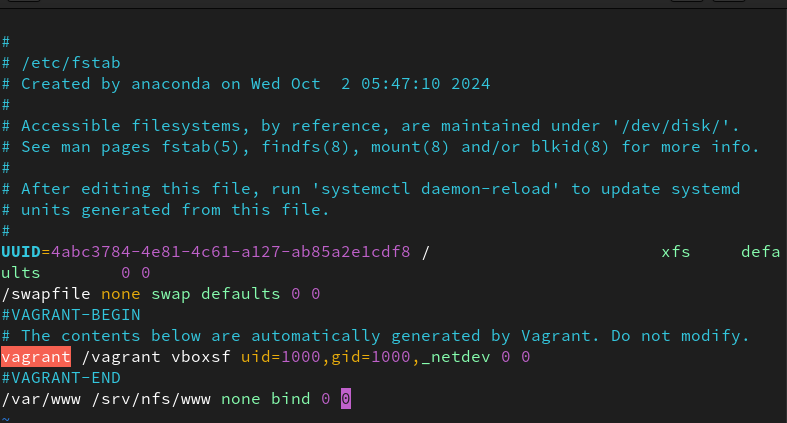
\includegraphics[width=\textwidth]{../images/image19.png}
    \captionof{figure}{Изменение файла /etc/fstab.}
    \label{img:19}
\end{center}

\item Повторно экспортировали каталоги, указанные в файле /etc/exports:
    \begin{minted}{bash}
exportfs -r
    \end{minted}
\item На клиенте проверили каталог /mnt/nfs (Рис. \ref{img:20}).

\begin{center}
    \centering
    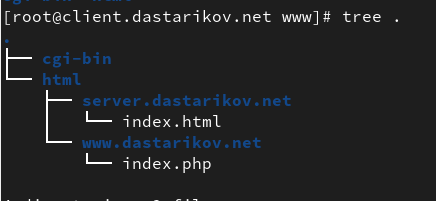
\includegraphics[width=\textwidth]{../images/image20.png}
    \captionof{figure}{Содержимое каталога /mnt/nfs/www.}
    \label{img:20}
\end{center}

\end{enumerate}

\subsection{Подключение каталогов для работы пользователей}
\begin{enumerate}
\item На сервере под пользователем dastarikov в его домашнем каталоге создали каталог common с полными правами доступа только для этого пользователя, а в нём файл dastarikov@server.txt (Рис. \ref{img:21}):
    \begin{minted}{bash}
mkdir -p -m 700 ~/common
cd ~/common
touch dastarikov@server.txt
    \end{minted}

\begin{center}
    \centering
    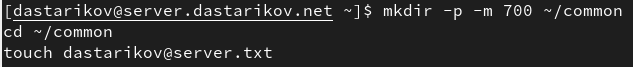
\includegraphics[width=\textwidth]{../images/image21.png}
    \captionof{figure}{Создание личного каталога common для пользователя dastarikov.}
    \label{img:21}
\end{center}

\item На сервере создали общий каталог для работы пользователя dastarikov по сети:
    \begin{minted}{bash}
mkdir -p /srv/nfs/home/dastarikov
    \end{minted}
\item Подмонтировали каталог common пользователя dastarikov в NFS:
    \begin{minted}{bash}
mount -o bind /home/dastarikov/common /srv/nfs/home/dastarikov
    \end{minted}
    Этот каталог имеет те же права доступа, что и локальный каталог common  (Рис. \ref{img:22}):

\begin{center}
    \centering
    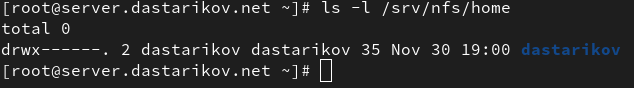
\includegraphics[width=\textwidth]{../images/image22.png}
    \captionof{figure}{Права каталога /srv/nfs/home/dastarikov.}
    \label{img:22}
\end{center}

\item Подключили каталог пользователя в файле /etc/exports, прописав в нём (Рис. \ref{img:23}):
    \begin{minted}{bash}
/srv/nfs/home/dastarikov 192.168.0.0/16(rw)
    \end{minted}

\begin{center}
    \centering
    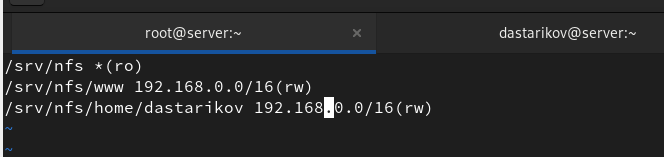
\includegraphics[width=\textwidth]{../images/image23.png}
    \captionof{figure}{Изменение файла /etc/exports.}
    \label{img:23}
\end{center}

\item Внесли изменения в файл /etc/fstab (Рис. \ref{img:28}):
    \begin{minted}{bash}
/home/dastarikov/common /srv/nfs/home/dastarikov none bind 0 0
    \end{minted}

\begin{center}
    \centering
    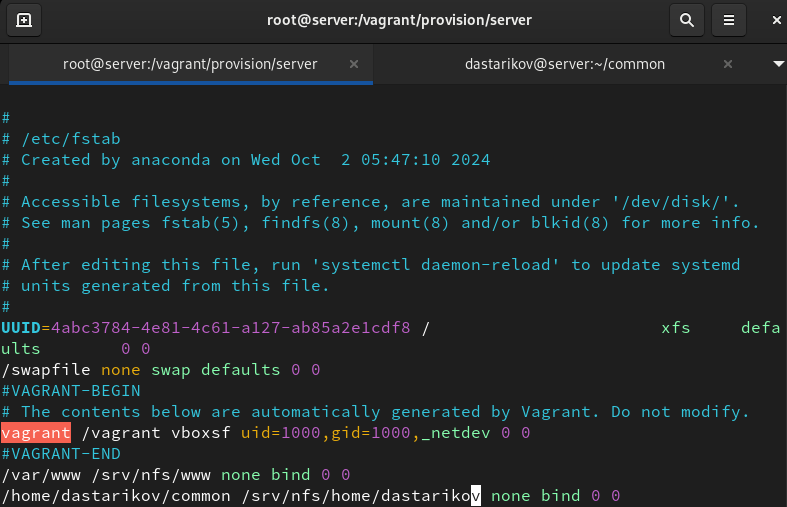
\includegraphics[width=\textwidth]{../images/image28.png}
    \captionof{figure}{Изменение /etc/fstab.}
    \label{img:28}
\end{center}

\item Повторно экспортировали каталоги:
    \begin{minted}{bash}
exportfs -r
    \end{minted}
\item На клиенте проверили каталог /mnt/nfs (Рис. \ref{img:24}).

\begin{center}
    \centering
    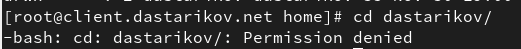
\includegraphics[width=\textwidth]{../images/image24.png}
    \captionof{figure}{Попытка зайти в каталог dastarikov на клиенте пользователем root.}
    \label{img:24}
\end{center}

\item На клиенте под пользователем dastarikov перешли в каталог /mnt/nfs/home/dastarikov и попробовали создать в нём файл dastarikov@client.txt и внести в него какие-либо изменения (Рис. \ref{img:29}):
    \begin{minted}{bash}
cd /mnt/nfs/home/dastarikov
touch dastarikov@client.txt
    \end{minted}

\begin{center}
    \centering
    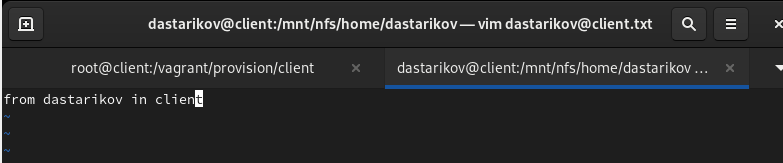
\includegraphics[width=\textwidth]{../images/image29.png}
    \captionof{figure}{Создание файла на клиенте.}
    \label{img:29}
\end{center}

Попробовали проделать это под пользователем root (Рис. \ref{img:24}).

\item На сервере посмотрели, появились ли изменения в каталоге пользователя /home/dastarikov/common (Рис. \ref{img:25}).

\begin{center}
    \centering
    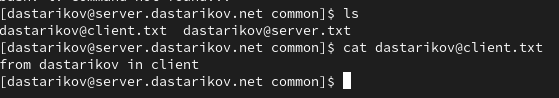
\includegraphics[width=\textwidth]{../images/image25.png}
    \captionof{figure}{Проверка изменений в локальном каталоге пользователя dastarikov.}
    \label{img:25}
\end{center}

\end{enumerate}

\subsection{Внесение изменений в настройки внутреннего окружения виртуальных машин}
\begin{enumerate}
\item На виртуальной машине server перешли в каталог для внесения изменений в настройки внутреннего окружения /vagrant/provision/server/, создали в нём каталог nfs, в который поместите в соответствующие подкаталоги конфигурационные файлы (Рис. \ref{img:26}):
    \begin{minted}{bash}
cd /vagrant/provision/server
mkdir -p /vagrant/provision/server/nfs/etc
cp -R /etc/exports /vagrant/provision/server/nfs/etc/
    \end{minted}
\item В каталоге /vagrant/provision/server создали исполняемый файл nfs.sh (Рис. \ref{img:26}):
    \begin{minted}{bash}
cd /vagrant/provision/server
touch nfs.sh
chmod +x nfs.sh
    \end{minted}
Открыв его на редактирование, прописали в нём следующий скрипт (вместо dastarikov укажите свой логин) (Рис. \ref{img:26}):
    \begin{minted}{bash}
#!/bin/bash
echo "Provisioning script $0"
echo "Install needed packages"
dnf -y install nfs-utils
echo "Copy configuration files"
cp -R /vagrant/provision/server/nfs/etc/* /etc
restorecon -vR /etc
echo "Configure firewall"
firewall-cmd --add-service nfs --permanent
firewall-cmd --add-service mountd --add-service rpc-bind --permanent
firewall-cmd --reload
echo "Tuning SELinux"
mkdir -p /srv/nfs
semanage fcontext -a -t nfs_t "/srv/nfs(/.*)?"
restorecon -vR /srv/nfs
echo "Mounting dirs"
mkdir -p /srv/nfs/www
mount -o bind /var/www /srv/nfs/www
echo "/var/www /srv/nfs/www none bind 0 0" >> /etc/fstab
mkdir -p /srv/nfs/home/dastarikov
mkdir -p -m 700 /home/dastarikov/common
chown dastarikov:dastarikov /home/dastarikov/common
mount -o bind /home/dastarikov/common /srv/nfs/home/dastarikov
echo "/home/dastarikov/common /srv/nfs/home/dastarikov none bind 0 0" >> /etc/fstab
echo "Start nfs service"
systemctl enable nfs-server
systemctl start nfs-server
systemctl restart firewalld
    \end{minted}

\begin{center}
    \centering
    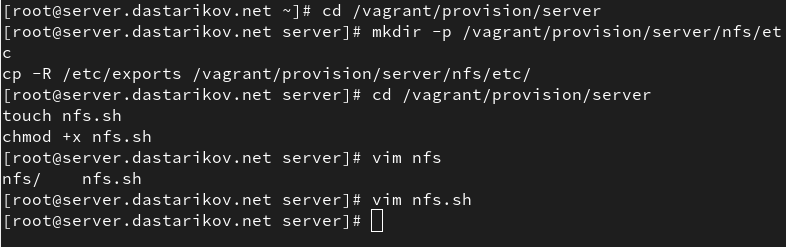
\includegraphics[width=\textwidth]{../images/image26.png}
    \captionof{figure}{Изменение настроек внутреннего окружения на виртуальной машине server.}
    \label{img:26}
\end{center}

\item На виртуальной машине client перейдите в каталог для внесения изменений в настройки внутреннего окружения /vagrant/provision/client/ (Рис. \ref{img:27}):
    \begin{minted}{bash}
cd /vagrant/provision/client
    \end{minted}
\item В каталоге /vagrant/provision/client создайте исполняемый файл nfs.sh (Рис. \ref{img:27}):
    \begin{minted}{bash}
cd /vagrant/provision/client
touch nfs.sh
chmod +x nfs.sh
    \end{minted}
Открыв его на редактирование, пропишите в нём следующий скрипт (Рис. \ref{img:27}):
    \begin{minted}{bash}
#!/bin/bash
echo "Provisioning script $0"
echo "Install needed packages"
dnf -y install nfs-utils
echo "Mounting dirs"
mkdir -p /mnt/nfs
mount server.dastarikov.net:/srv/nfs /mnt/nfs
echo "server.dastarikov.net:/srv/nfs /mnt/nfs nfs _netdev 0 0" >> /etc/fstab
restorecon -vR /etc
    \end{minted}

\begin{center}
    \centering
    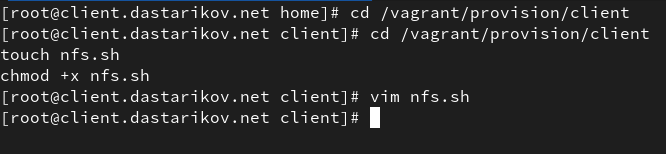
\includegraphics[width=\textwidth]{../images/image27.png}
    \captionof{figure}{Изменение настроек внутреннего окружения на виртуальной машине client.}
    \label{img:27}
\end{center}

\item Для отработки созданных скриптов во время загрузки виртуальных машин server и client в конфигурационном файле Vagrantfile необходимо добавить в соответствующих разделах конфигураций для сервера и клиента:
    \begin{minted}{bash}
server.vm.provision "server nfs",
type: "shell",
preserve_order: true,
path: "provision/server/nfs.sh"
client.vm.provision "client nfs",
type: "shell",
preserve_order: true,
path: "provision/client/nfs.sh"
    \end{minted}

\end{enumerate}

\section{Выводы}
В результате лабораторной работы познакомились с настройкой сервера NFS на примере создания каталога веб-сервера и каталога для удаленной работы конкретного пользователя.
\end{document}
